\section{Neuronale Netze - kurzer Überblick}
\label{sset:neuronale-netze-kurzer-überblick}
\textbf{Wieso werden neuronale Netze verwendet?}
\begin{itemize}
	\item Massive parallelism.
	\item Massive constraint satisfaction for ill-defined input.
	\item Simple computing units.
	\item Many processing units, many interconnections.
	\item Uniformity (-> sensor fusion)
	\item Non-linear classifiers/ mapping (-> good performance)
	\item Learning/ adapting
	\item Brain like ??
\end{itemize}
\textbf{Wofür werden neuronale Netze verwendet?}
\begin{itemize}
	\item Classification
	\item Prediction
	\item Function Approximation
	\item Continuous Mapping
	\item Pattern Completion
	\item Coding
\end{itemize}
\textbf{Welche Kriterien müssen beim Entwurf von neuronalen Netzen beachtet werden?}
\begin{itemize}
	\item Recognition Error Rate
	\item Training Time
	\item Recognition Time
	\item Memory Requirements
	\item Training Complexity
	\item Ease of Implementation
	\item Ease of Adaptation
\end{itemize}
\textbf{Welche Parameter werden typsicherweise vom Entwerfer bestimmt?}
\begin{itemize}
	\item Net Topology
	\item Node Characteristics
	\item Learning Rule
	\item Objective Function
	\item (Initial) Weights
	\item Learning Parameters
\end{itemize}
\textbf{Wo werden neuronale Netze verwendet?}
\begin{itemize}
	\item Space Robot*
	\item Autonomous Navigation*
	\item Speech Recognition and Understanding*
	\item Natural Language
	\item Processing*
	\item Music*
	\item Gesture Recognition
	\item Lip Reading
	\item Face Recognition
	\item Household Robots
	\item Signal Processing
	\item Banking, Bond Rating
	\item Sonar
\end{itemize}
\textbf{Advanced Neural Models}
\begin{itemize}
	\item Time-Delay Neural Networks (Waibel)
	\item Recurrent Nets (Elman, Jordan, Robinson,..)
	\item Higher Order Nets
	\item Modular System Construction
	\item Adaptive Architectures
	\item Hybrid Neural/Non-Neural Architectures
	\item Deep Nets
\end{itemize}
\textbf{Welche Probleme können beim Entwurf von neuronalen Netzen auftreten?}
\begin{itemize}
	\item Local Minima
	\item Speed of Learning
	\item Architecture must be selected
	\item Choice of Feature Representation
	\item Scaling
	\item Systems, Modularity
	\item Treatment of Temporal Features and Sequences
\end{itemize}
\textbf{Eigenschaften von neuronalen Netzen:}
\begin{itemize}
	\item non-linear classifier
	\item approximate posterior probability
	\item non-parametric training
\end{itemize}
\newpage

\section{Pattern Recognition}
\label{sect:pattern-recognition}
\begin{figure}[h]
	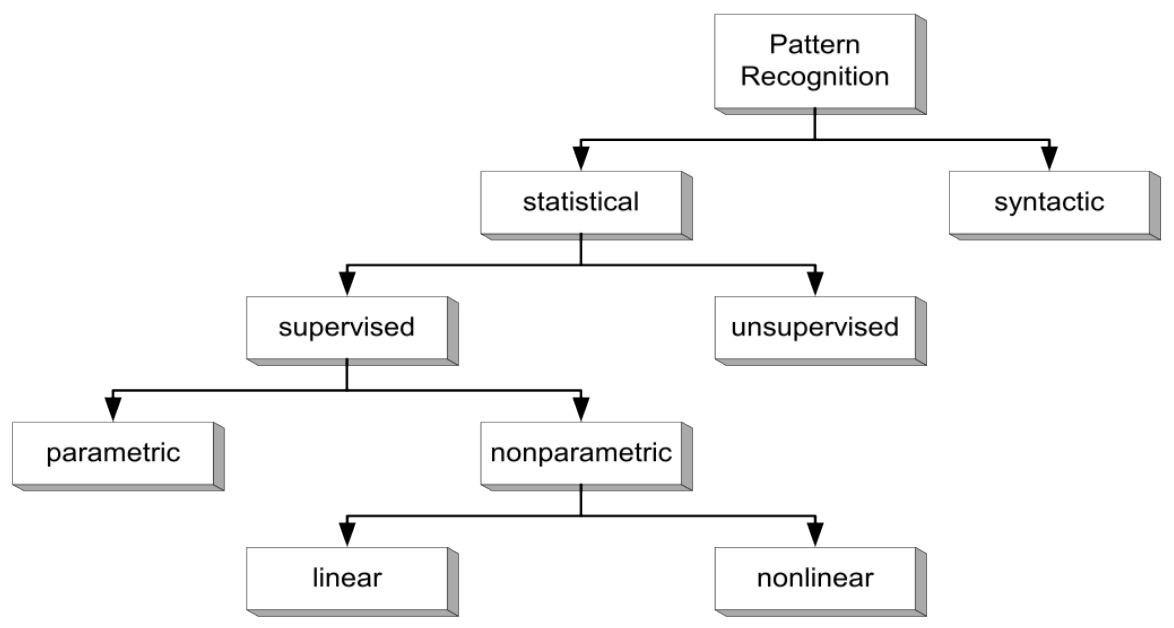
\includegraphics[scale=0.3]{pattern-recognition-partitioning}
\end{figure}

\begin{itemize}
	\item supervised:
		\begin{itemize}
			\item labels / classes of training data are known
			\item train a classifier
		\end{itemize}
	\item unsupervised:
		\begin{itemize}
			\item labels / classes are not known
			\item find the structure of the data
			\item methods: clustering, autoassociative nets
		\end{itemize}
	\item parametric:
		\begin{itemize}
			\item assume underlying probability distribution
			\item estimate the parameters
			\item eg.: Gaussian classifier
		\end{itemize}
	\item unparametric:
		\begin{itemize}
			\item doesn't assume underlaying probability distribution
			\item estimate probability of error from training data
			\item nearest neighbours, parzen window, perceptron
		\end{itemize}
\end{itemize}

\subsection{Bayes Decision Theory - Parametric}
\label{ssect:bayes-decision-theory}
\begin{align*}
P(\omega_j |x) &= \frac{p(x|\omega_j) \cdot P(\omega_j)}{p(x)} \\
p(x) &= \sum_j p(x|\omega_j) \cdot P(w_j)
\end{align*}
Since we have overlapping probability distribution false classifications occur. Simply speaking to reduce false classification always decide for the class with the highest probability (errors still can occur!).

\subsection{Classifier Discrimination Function}
\label{ssect:classfier-discrimination-function}
The \textit{classifier discrimination function} iterats over all classes and choses those which has the highest probability. In the case of the Gaussian classifier it looks as follows:
\begin{align*}
g_i &= P(\omega_i | x) \\
&= p(x | \omega_i) \cdot P(\omega_i) \\
&= \log(p(x | \omega_i)) + \log(P(\omega_i))
\end{align*}
Problems:
\begin{itemize}
	\item limited traning data
	\item limited computation
	\item class-labeling potentially costful and errorful
	\item classes or features might not be known
\end{itemize}
Parametric solution: assume that $p(x|\omega_i)$ has a parametric form. The most common representative: multivariant normal density.\\
Univariant normal density:
\[
p(x) = \frac{1}{\sqrt{2 \cdot \pi \sigma}} \cdot e^{(-\frac{1}{2} \cdot \frac{x - mu}{\sigma})^2}
\]
Multivarian normal density:
\[
p(\overleftarrow{x}) = \frac{1}{\sqrt[d]{2 \pi} \cdot \sqrt{|\Sigma|}} \cdot e^{-\frac{1}{2} \cdot \frac{(\overleftarrow{x} - \overleftarrow{\mu})^2}{\Sigma}}
\]
The following form takes effect for the classifier discrimination function:
\[
g_i(\overleftarrow{x}) = -\frac{1}{2} \cdot \frac{(\overleftarrow{x} - \overleftarrow{\mu_i})^2}{\Sigma_i} - \frac{d}{2} \cdot \log(2\pi) - \frac{1}{2} \cdot \log(|\Sigma_i|) + \log(P(\omega_i))
\]
For the Gaussian classifier we have to estimate the \textit{covariance matrix} $\Sigma_i$ and the \textit{mean vector} $\mu_i$. To estimate the parameters we can use the \textit{MLE: maximum likelihood estimation} for the univariant case.
For the multivariant case we can use:
\[
\overleftarrow{\mu} = \frac{1}{N} \cdot \Sigma_{k = 1}^{N} \overleftarrow{x_k}
\]
\[
\Sigma = \frac{1}{N} \cdot \Sigma_{k = 1}^{N} (\overleftarrow{x_k} - \overleftarrow{\mu}) \cdot (\overleftarrow{x_k} - \overleftarrow{\mu})^T
\]
\subsection{Curse of Dimensionality}
\label{ssect:curse-of-dimensionality}
The problem with the classifier design in general is that we can not say which features are the most valuable ones, are more features better and is features are useful will they be ignored? \\
However in general we can say that more features performe worse because we have limited training data and we still have to estimate the parameters (Eg. 1000 sample training data and 1000 parameters to estimate). We have to select the best feature and might have to reduce the dimensions (for example with the \textit{Principle Component Analysis (PCA)}.

\subsubsection{Principle Component Analysis (PCA)}
\label{sssect:principle-component-analysis-pca}
The idea is that single dimension are correlated and we want to remove the dimension with the least informations:
\begin{itemize}
	\item[1.] find the axis with the highest variance
	\item[2.] rotate the space along the axis
	\item[3.] not the dimensions are uncorrelated
	\item[4.] remove the dimension with the lower variance
\end{itemize}

\subsection{Non-Parametric Methods}
\label{ssect:non-parametric-methods}
\textit{Non-Parametric Methods} do not assume any distributions and try to find structures in the data itself.

\subsubsection{Parzen Window}
\label{sssect:parzen-window}
\begin{itemize}
	\item[1.] chose a window with volume $V$
	\item[2.] count the numbers of samples in that window $p(x) = \frac{\frac{k}{N}}{V}$ where $k$ are the samples in the window and $N$ is the total numbers of samples.
\end{itemize}
The hard part is to chose the window size. the thumb roule is: $V_n = \frac{1}{\sqrt{n}}$

\subsubsection{k-nearest Neighours}
\label{sssect:k-nearest-neighbours}



\newpage